

\begin{example}\label{ex:PermuteScopeShallowFold}
The function
\begin{align*}
\ranked{\reduce k \Sigma\cdot \Gamma\to \reduce k (\Sigma\cdot \Gamma)}
\end{align*}
which puts shallow composition inside the scope of the fold is derivable. Indeed, it is the composition of the following functions:
\begin{align*}
\ranked{\reduce k \Sigma\cdot \Gamma\to \reduce k \Sigma\cdot \reduce k\Gamma^k\to \reduce k(\reduce k \Sigma\cdot \Gamma^k)\to \reduce k (\Sigma\cdot \Gamma)}
\end{align*} 
\end{example}

One annoying thing about the unfold function and the function that reduces the degree of the fold
\begin{align*}
\ranked{\tmonad \reduce k \Sigma \to \reduce k \tmonad \Sigma\cdot  \tmonad \reduce k \Sigma \qquad \reduce k\Sigma \to \reduce {k-l} {(\Sigma\cdot(0+1))}}
 \end{align*}
 is that they append a type after a $\cdot$. In our futur developments, we will need to derive functions of the form
 \begin{align*}
 \ranked{\Gamma\cdot\Delta\to \Gamma}
 \end{align*}
 to get rid of these appended types. Obviously, functions of this type are not derivable for any $\rGamma$ and $\rDelta$. We show in the following some situations where it becomes derivable.
 
 \begin{example}
 Suppose that $\rSigma$ is a ranked set containing a binary and a nullary element. We can derive a function
 \begin{align*}
\ranked{\tmonad\Sigma\cdot\Gamma\to \tmonad\Sigma}
 \end{align*}
 as the composition of the following functions:
 \begin{align*}
\ranked{\tmonad\Sigma\cdot\Gamma\to \tmonad\Sigma\cdot\bot\to\tmonad\Sigma\cdot\tmonad(0+2)\to \tmonad(\Sigma+0+2) \to \tmonad\Sigma} 
 \end{align*}

Suppose that $\rGamma, \rDelta$ are two types such that we can derive a function of type 
 \begin{align*}
 \ranked{\Gamma\cdot\Delta\to \Gamma}
 \end{align*}
Then we can also derive a function of type 
\begin{align*}
\ranked{\reduce k \Gamma\cdot\Delta\to \reduce k \Gamma}
\end{align*}
using the following derivation. 
\begin{align*}
\ranked{\reduce k \Gamma\cdot\Delta\xrightarrow{Ex.~\ref{ex:PermuteScopeShallowFold}} \reduce k (\Gamma\cdot\Delta) \to \reduce k \Gamma}
\end{align*}
Similarly, we can derive a function of type
\begin{align*}
\ranked{ \Gamma^k\cdot\Delta\to \Gamma^k}
\end{align*}
using the following derivation. 
\begin{align*}
\ranked{\Gamma^k\cdot\Delta\to (\Gamma\cdot\Delta)^k \to \Gamma^k}
\end{align*}
Using these functions, when we will want to reduce the degree of a fold of a type $\ranked{\tmonad\Sigma}$, $\ranked{(\tmonad\Sigma)^k}$, etc, we will use the following functions instead of the basic ones:
\begin{align*}
\ranked{\reduce l\tmonad \Sigma\to \reduce {l-m}(\tmonad \Sigma\cdot(0+1))\to \reduce {l-m}\tmonad \Sigma }\\
\ranked{\reduce l(\tmonad \Sigma)^k\to \reduce {l-m}((\tmonad \Sigma)^k\cdot(0+1))\to \reduce {l-m}(\tmonad \Sigma)^k }
\end{align*} 
\end{example}


\begin{example}[Partial shallow unfold]~\label{ex:PartialShallowUnfold}
We need a "partial shallow unfold"
\begin{align*}
\ranked{\reduce k \Sigma\cdot (1+\Gamma^k)\to \reduce k (\Sigma\cdot(1+\Gamma))}
\end{align*}
\begin{center}
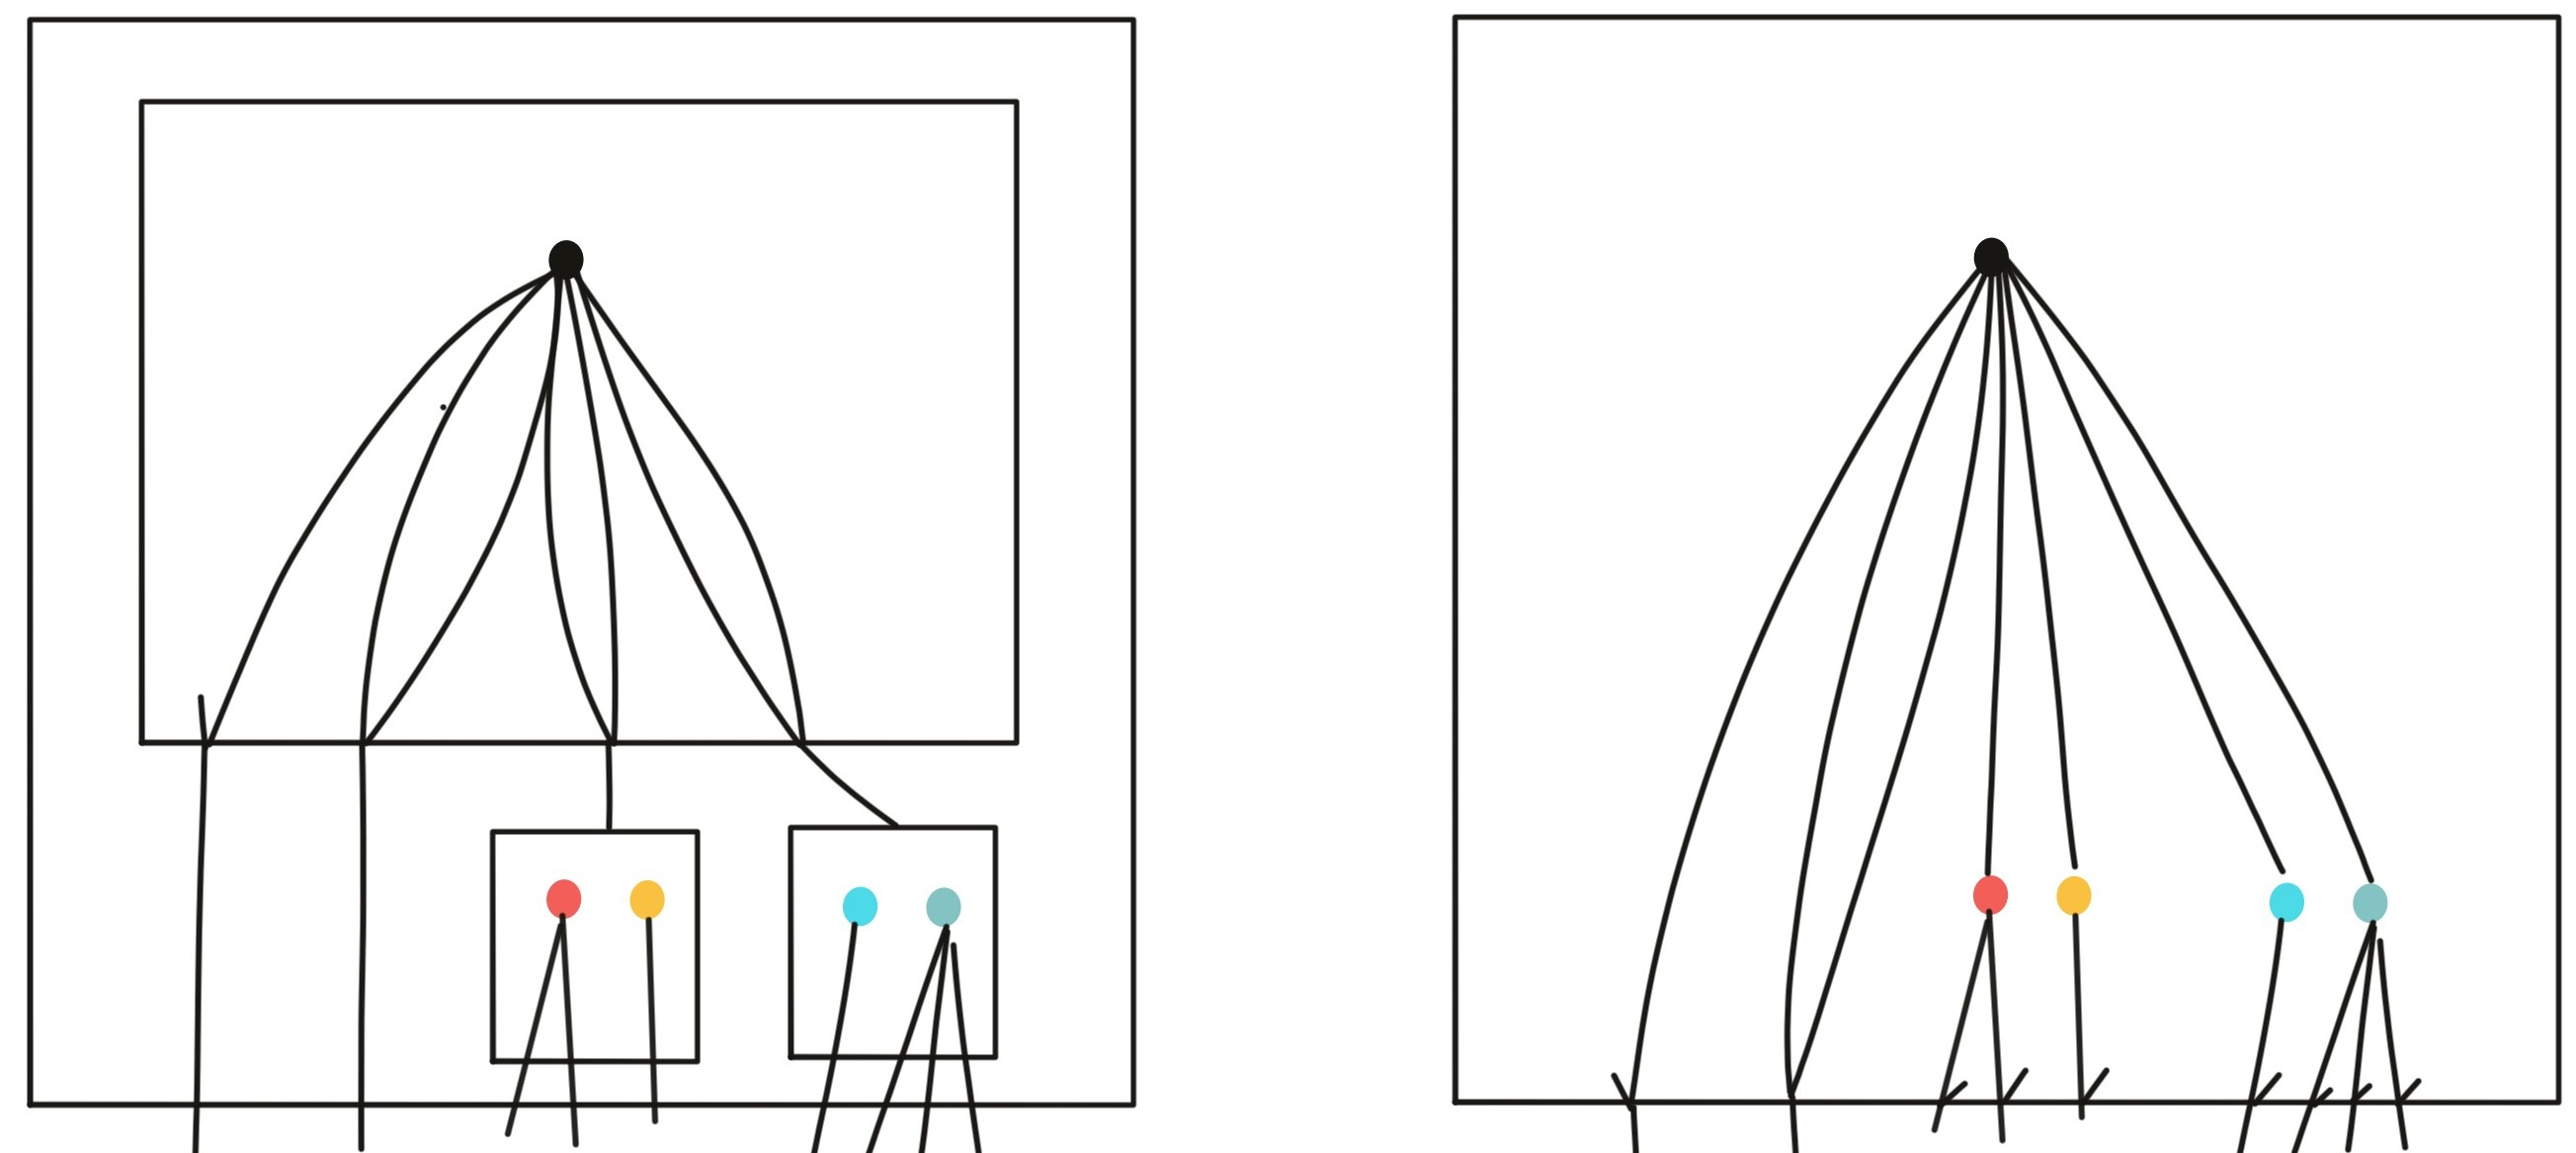
\includegraphics[scale=.09]{MyPicPartialShallowUnfold.jpg}
\end{center}
This function can be derived as follows. First we lift the functions
\begin{align*}
\ranked{1\to \reduce k 1^k}\qquad \text{ and } \qquad\ranked{\Gamma^k\to \reduce k\Gamma^k}
\end{align*}
obtaining the function
\begin{align*}
\ranked{\reduce k \Sigma\cdot (1+\Gamma^k)\to \reduce k \Sigma\cdot (\reduce k 1^k+\reduce k\Gamma^k) }
\end{align*}
We compose the result with the following  (series of) injections
\begin{align*}
\ranked{\reduce k \Sigma\cdot (\reduce k 1^k+\reduce k\Gamma^k)\to \reduce k \Sigma\cdot \reduce k (1+\Gamma)^k}
\end{align*}
Finally we permute the fold with the shallow product, then we apply the shallow unfold to obtain the result.
\end{example}
